\clearpage
\section{Visualizing Windows System Traces}
\label{sec:lviz}

% \mypreamble{
% This section presents \code{lviz}, which uses Windows system traces
% to study program behaviours including patterns, anomalies,
% faults and other problems.
% The collaborative work has been published in \cite{wu2010visualizing}.
% The author of this thesis focuses on log processing and case study.
% The DotPlot algorithm (Section~\ref{sec:lviz-imp}) is implemented
% by other collaborators.
% }

% \subsection{Introduction}

Software is increasingly complex with many interactions with other software
and the operating system.
The previous visualization shows the complexity in the
aspect of module dependency.
Other factors include persistent state interaction, inter-process communication,
networking, etc.
This complicates understanding software/component behavior and diagnosing
problems or performance.
As discussed in Section~\ref{sec:bg-win},
the close source nature of Microsoft Windows (or simply, Windows)
exemplifies this trend.
Suppose our task is to understand/diagnose/debug some software on Windows.
Ideally, system/software documentation or source code
analysis would give the answer.
In practice, however, this may not be
workable either due to lack of source or overall
system complexity being too high.
An orthogonal approach to address this issue is by examining
detailed system behavior.
Recently, there are a number of monitoring systems which
give detailed system traces such as DTrace~\cite{cantrill2004dynamic} for Solaris,
DProbes for Linux and Flight Data Recorder~\cite{verbowski6flight}
and WinResMon (Sec.\ref{sec:winresmon}) for Windows.
However, as shown earlier in this chapter,
the system traces can be very large and also
difficult to analyze.

We propose \code{lviz}, a visualization tool for
understanding such large and complex system traces.
\code{lviz} has a number of visualizations.
In the thesis, we focus on the visualization which we call VDP.
It consists of a number of inter-connected sub-visualizations:
an extended DotPlot;
two Axis Histograms; and one or more barcodes.
The VDP can be flexibly configured for different purpose.
In Section~\ref{sec:lviz-vis}, we show the design and configurations of VDP.
In Section~\ref{sec:lviz-imp}, we show that
the prototype of \code{lviz} is efficient and can handle large system traces
with real-time response. For example, a trace of size 120MB with 558K events 
is loaded in under 3 seconds
and after that it can be interactively displayed/zoomed in around 0.5 seconds.
The VDP can be used on different traces and for different purpose
by using different configurations.
In Section~\ref{sec:lviz-study}, we use some case studies to show that
VDP can be used for solving performance problems,
program failure diagnosis and finding execution patterns/anomalies.

\subsection{Related Work}
\label{sec:lviz-related}

% \TODO{maybe dont need the first para}
% There are a number of related works on execution trace visualization,
% some are graph based, some are hierarchical,
% some are Cartesian coordinate based.
% We focus on Cartesian coordinate base visualization to which VDP belongs.
% The Cartesian coordinate based visualization is commonly used when each
% visualized entity (function, event, object, line of source code, etc.)
% is associated with some numerical properties.
% Each entity is then positioned on to the Cartesian coordinate based on
% its properties.

% \TODO{reviewer 2:
% The statement in section 2 that Cartesian visualizations are commonly used
% when each visualized entity is associated with two or three numerical
% properties is somewhat confusing. The choice of the so-called embedding, or
% projection, is in Infovis in general not one-to-one to the data attributes,
% at least not at this level. For example one would visualize some data using
% hierarchies primarily and not Cartesian plots if the most important aspect to
% reason about is the hierarchical one, even when the data has 2 or 3 numerical
% attributes per element. Or a table in a data base can be shown as a table,
% but better as a graph, if it actually encodes a graph. I think strongly that
% the layout choice should reflect the task at hand, and not data modeling
% issues.  fixed.
% }

% \TODO{reviewer 2:
% In the previous work you should definitely discuss the more recent work of
% Holten, Cornelissen, van Deursen, and Zaidman on visualizing trace
% information, see "Understanding Execution Traces Using Massive Sequence and
% Circular Bundle Views" (proc. ICPC 2007), since it is at least as related to
% the topic of this paper as the other references, and is quite recent. The
% work of F. van Ham and J. Abello on MatrixZoom fits also in this area.  fixed
% (only added the first paper).
% }

SeeSoft~\cite{eick1994graphical} visualizes general log files by zooming out
lines of text logs and coloring them by message types.
SeeLog~\cite{eick1996displaying} visualizes Unix accounting trace files by
plotting events by time and process.
SeeLog can be viewed as a restricted variant of the
VDP visualization.
Magpie~\cite{barham2004using} is a performance analysis tool designed for web
servers.
It uses collected system events including file I/O, computation,
thread scheduling and network to analyze the resources usage of
HTTP requests.
BootVis~\cite{bootvis} 
is a visualization tool to tune
Windows booting plotting resource use versus time.

Bodic et al.~\cite{bodik2005combining} propose another visualization tool for
web servers.
It shows frequency of different HTTP requests
and highlight anomalies that may indicate site failures.
VDP on the other hand is a general trace visualizer but
it can be used for similar diagnosis (see Sec.~\ref{sec:wbbench}).
TuningFork~\cite{bacon2007tuningfork} is a trace analysis tool for real-time
systems including visualizing unsatisfied real time constraints in real-time
systems.

EVolve~\cite{wang2003evolve} is a visualization framework for understanding
Java program by visualization execution traces from the JVM and
has a DotPlot visualization.
% It includes a DotPlot module which has some similarity with VDP.
However, VDP uses an extended DotPlot (see Sec.~\ref{sec:lviz-vis})
and generates different visualizations (see Fig.~\ref{fig:make-matching})
depending on its configuration.
\code{lviz} is designed to scale for large traces and
to be efficient to meet user interaction needs.
Voigt et al.~\cite{voigt2009object} propose a visualization method which correlates
class method invocation, object invocation and time.
To correlate methods and objects, it places objects and methods
on each axis and draw dots to represent the
method-access-object relationship.
Cornelissen et al.~\cite{cornelissen2007understanding} propose two visualizations,
massive sequence and circular bundle views, to examine execution traces.
The massive sequence view visualizes a trace by placing each event as rectangles
according to its invoking software module (X-axis) and time (Y-axis).
The circular bundle view visualizes software module interactions by arranging
modules into a tree and draw two-module interaction as a curve along the
path in the tree.
These visualizations are different as they do not compare events 
nor work with closed source software.

% \TODO{reviewer 3:
% Dotplots and their extensions have been studied in the field of visualization
% more than extensively. They have been proven to be useful for finding
% patterns in similarities in various fields. In this paper, the dotplot is not
% used differently. The configuration of visualizations reminds me DNAVis: Case
% Study: Visualization of annotated DNA sequences, Tim Peeters, Mark Fiers,
% Huub van de Wetering, Jan-Peter Nap, Jarke J. van Wijk, Joint Eurographics
% IEEE TCVG Symposium on Visualization (2004).
% }

\subsection{System and Visualization Design}

% \TODO{reviewer 3:
% Look at the order of the figures, they do not appear in the same order as they appear in the
% text. Also, they are not as close as possible to the reference in the text.
% }

We describe the design of \code{lviz}, a system for visualizing Windows system
traces.
% \footnote{
% \code{lviz} has a number of visualizations. In this work, we focus on the VDP
% visualization.
% }
We emphasize that the visualization proposed
is not specific to Windows as traces from other operating systems
can be used as well.
\code{lviz} can be easily adapted to read traces in other format,
which make it friendly to other monitoring systems such as DTrace
and SystemTap.

\subsubsection{System Traces}
\label{sec:systrace}

Our objective is to visualize detailed system traces.
In the rest of the section, we will shorten system trace to simply trace.
Our traces are obtained with WinResMon (Section~\ref{sec:winresmon}) which
captures all operations performed by the Windows kernel
from all processes.
% Our aim is to capture the relevant operations which can be attributed
% to interactions between software (system and applications).
% Collecting trace events in Windows is much harder than UNIX.
% Windows NT (Server 2000, XP, Server 2003, Vista) is a microkernel
% based operating systems.
% Programs are usually written for the Win32 API but those are decomposed
% into microkernel operations.
% However, as Windows is closed source,
% only the Win32 API is documented and not the microkernel API.
% We use WinResMon~\cite{ramnath2006winresmon} to capture system trace.

A WinResMon trace consists of four classes of events
due to operations on processes, files, network and the registry.
An event contains the following properties: (the example events
in Figure~\ref{fig:logex} use the ordering below)
\begin{tightitemize}
\item {\bf PID/TID} is the ID of the process/thread which
performs the operation.
%Since it is reusable, it is not unique over time.
\item {\bf Program name} is the pathname of the program binary.
%\item {\bf Group name and User name} is the owner of the process.
\item {\bf Group} and {\bf User name} of the process.
%Unlike UNIX, in Windows there are multiple privileged users.
% where root is the only privileged user,
% in Windows there are more than one privileged user, such as
% ``{\tt NT AUTHORITY\BS SYSTEM}'',
% ``{\tt NT AUTHORITY\BS LOCAL SERVICE}'',
% ``{\tt NT AUTHORITY\BS NETWORK SERVICE}''
% and arbitrary number of administrators.
\item {\bf Start and end times} of the event.
% are 64-bit timestamps derived from the Intel processor performance counters.
% % are 64-bit timestamps generated by the RDTSC~\cite{rdtsc} instruction.
% % \TODO{This timestamp is a relative timestamp counting from CPU reset.
% % CPU reset may be triggered by system boot or waking up from hibernate,
% % thus one has to add addition bits to ensure monotone increasing timestamp.}
% \TODO{usenix comm:
% A minor technical tidbit: in Section 3.1 it is said that start and end time of
% the event is recorded using CPU perf counters; what happens in SMPs? How is
% the timestamp decided?}
\item {\bf Operation type} is specific to the event.
Some examples are given below.
\item {\bf Operation parameters}: The semantics depends on the operation type,
e.g.  resource pathname, file access flags, etc.
% and I/O data.
%Collecting I/O data can be turned on/off by command line options,
%as it is comparably expensive.
%The maximum size of I/O data can also be adjusted.
\item {\bf Return value} from the operation
is either success or an error number explaining why the operation failed.
\item {\bf Call stack trace} of the process which generated the event.
In this work, we use the deepest function call
from the corresponding executable, i.e.
excluding functions in libraries,
but one could also use the full stack trace.
This information is useful to associate a program point in the
application code with the event.
\end{tightitemize}

% There are 46 operation types in total, 6 related to file,
% 7 related to registry, 5 related to process, and 28 related to network.
Examples of events are file operations,
e.g.  file\_create, file\_close and file\_read;
registry operations, e.g. reg\_setvalue;
process operations, e.g.  thread\_create;
and network operations, e.g. socket\_bind.
Pathnames of files and registry keys are recorded as operation parameters.
Additional information depending on the specific operation is also recorded.
For example, file\_create, which represents both opening an existing file
and creating a new file, the operation parameters include the pathname of
the opened or created file, access flags, file attributes, creation disposition
(create new, open existing,
% truncate existing, or append to existing files),
etc.) and other Windows operating system specific information.
Figure~\ref{fig:logex} shows two examples of events.
WinResMon can optionally capture the data associated with an
event. (see Section~\ref{sec:wbbench} which uses network packet data)
% While file and registry resources are represented as paths,
% network resources are represented as network address, i.e. IP address and port.
% Only TCP and UDP protocols are recorded.
% A socket is not associated with an address until {\tt bind()} or {\tt connect()} is called,
% Thus not all network operations are associated with resources.

\begin{figure}
\fbox{\parbox{0.95\columnwidth}{
\tt\small
1268 1732
"C:\BS WINDOWS\BS System32\BS svchost.exe" "NT AUTHORITY\BS SYSTEM"
1098307213586 1098307319878
file\_create
"\BS Device\BS HarddiskVolume1\BS WINDOWS\BS Prefetch\BS NET1.EXE-029B9DB4.pf"
access=0x120089, share=0x0, attr=0x0, cd=0x1, co=0x60, si=0x1
STATUS\_SUCCESS
\vspace*{1mm}

\hrule
\vspace*{1mm}

204 960
"C:\BS WINDOWS\BS system32\BS cmd.exe" "GROUP\BS USER"
1101551207684 1101551216008
reg\_queryvalue
"\BS Registry\BS Machine\BS Software\BS Policies\BS Microsoft\BS Windows\BS Safer\BS CodeIdentifiers"
handle=0x78, name="LogFileName", t=0x0, l=0
STATUS\_OBJECT\_NAME\_NOT\_FOUND
}}
%\caption{Two examples of events (without call stack trace)}
\caption{Two examples of events}
\label{fig:logex}
\end{figure}

% A system trace is stored in a compressed text file, where each line
% records an event.
% We choose this format because it makes filtering and processing easy through
% existing UNIX stream text processing programs.
% The drawback of text file is the difficulty in random accessing,
% however, our visualization programs are implemented to sequentially
% access the trace.

% \TODO{reviewer 3:
% The list in section 3.1 can be compressed and figure 1 can be given inline.
% }

\subsubsection{Trace Visualization}
\label{sec:lviz-vis}

Visualizations for traces need to be able to compress a lot of detail
and yet be usable for illustrating many different
kinds of system behavior ranging from understanding
system administration to debugging to performance evaluation.
% investigating security issues, comparing behavior of program versions, etc.
In order to meet such a wide range of needs, we will see that the visualization
should be adaptable and configurable to show specific aspects for a
given purpose.  It must also be able to scale at different detail levels.

% We describe the design and rationale
% of two novel visualizations: RTG and Extended DotPlot.
% They have different purposes and complement each other.
% Both visualizations are meant for interactive use for exploring different
% ways of looking at the same trace under different visualization
% configurations and zoom levels.
% % modes which also includes
% % interactive zooms to see finer detail.

Our visualizations use color for greater visual
bandwidth as well as customization flexibility.
We support both RGB and CMY color modes.
The RGB color mode displays events on a black background
and is appropriate if the visualization is displayed on monitors to
make it easy to see events.
For printed output, a CMY mode, which uses subtractive color,
tends to be easier to see.
In the thesis, being in print format, we use the CMY mode
and try to minimize the use of yellow due to its closeness to white.
% \footnote{
% % (In \code{lviz} switching between RGB and CMY
% % gives RGB:white $\mapsto$ CMY:black, RGB:red $\mapsto$ CMY:cyan, etc.)
% % In the thesis, all figures and illustrations use the CMY color model,
% In CMY, the primitive colors are $cyan$, $magenta$ and $yellow$,
% and the composition rules are:
% $cyan+magenta=blue$;
% $cyan+yellow=green$;
% $magenta+yellow=red$; and
% $cyan+magenta+yellow=black$.
% }
% When referring to specific colors generated in
% a visualization, we may specify the color model to
% avoid confusion, e.g. CMY:yellow.
% The RGB color model is better for showing
% detail since it's easier to see color
% pixels on black than it is to see light color print on white paper.
% Since color in RGB is additive,
% it is also more intuitive for reasoning.
% % and the processing algorithms in \code{lviz} mainly employ 24-bit RGB.
%We highlight that the reader can see
%more detail in the PDFs by zooming in.


% \TODO{
% eurosys comments:
% It is a bit confusing that DotPlots are presented as normally having white
% for matches, but it seems that in your approach there are colors for
% matches.  Perhaps this should be explained more explicitly.
% }

A {\em binary DotPlot} is a black \& white image
where each axis denotes a sequence of events.
The color of a dot (or pixel) at position ($i$,$j$) is black
when the two events at position $i$ and $j$ from the corresponding sequence
match, and white otherwise.
%\footnote{
%As the print figures are on paper, the CMY mode uses black for a match
%and white for the background. This would be reversed in RGB mode.
%}
The rationale for a binary DotPlot is to visualize event similarity
between two sequences.
It has been used for comparing DNA sequences \cite{maizel1981enhanced},
visualizing the structure of music \cite{foote1999visualizing}
and investigating data formats and binaries \cite{kaminsky2006black}.
DotPlots can be used to do self-comparison
by comparing a sequence with itself or to compare
two different sequences.

\begin{figure}[tb]
\begin{center}
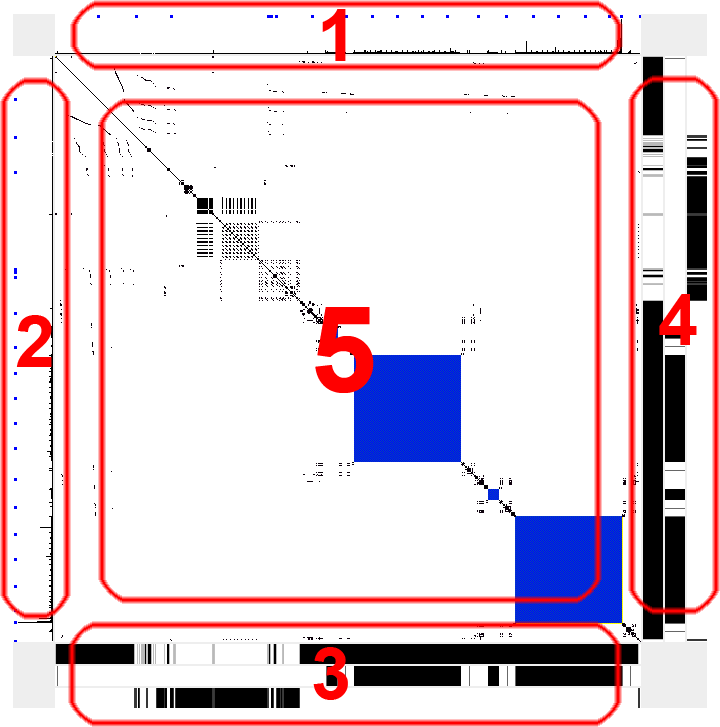
\includegraphics[width=0.4\textwidth]{lviz/elements.png}
\caption{Elements of VDP: axis histograms (Region 1,2);
barcodes (3,4); and extended DotPlot (5). This figure is same as
Figure~\ref{fig:cp-xcopy} with the added annotation.}
\label{fig:elements}
\end{center}
\end{figure}

Here, we develop a novel DotPlot based visualization which is
extensible and can be configured for many uses.
Our visualization, which we call {\em VDP},
consists of a number of sub-visualizations:
an {\em extended DotPlot} (or simply, DP in the rest of the section), two
Axis Histograms, and some barcodes.
% We now describe the elements of VDP.
Figure~\ref{fig:elements} gives an overview of all the elements:
$(i)$ the DP (region 5);
$(ii)$ the x-axis histogram (region 1) and
y-axis histogram (region 2);
and $(iii)$ the x-axis barcodes (region 3) and
y-axis barcodes (region 4).
A larger diagram of the same visualization highlighting various
details is in Figure~\ref{fig:cp-xcopy}.

An important aspect of the VDP is that it is intended to
be extensively customizable. Thus, it gives rise to a family of visualizations.
In Section~\ref{sec:lviz-study}, we show how to apply and customize
the VDP for different purposes. The elements of a VDP as follows.

{\bf DP}:
% We overload the DotPlot (DP) to refer either to our
% entire DotPlot visualization or to the extended DotPlot graphic.
Our DP visualization extends a binary DotPlot in a number of ways.
Since a trace can be long, several events are aggregated
together into a single pixel in a window.
DotPlots which contains aggregated events are drawn as grayscale images
which are then colored using the DP coloring rules for customizing
the appearance.
Normalization or histogram equalization (see Section~\ref{sec:lviz-imp})
is applied on the image so that the color intensity fits in a displayable range.
Our extended DotPlots (see region 5 in the center of Figure~\ref{fig:elements})
can be drawn with event-ordering, time-ordering or time-duration-ordering.
In an {\em event-ordered} DP, the events are plotted in
sequence as they occur in the trace.
In a {\em time-ordered} DP, the events are plotted in time order
according to the start time of the event.
Furthermore, each pixel in the visualization can contain several events
as there may be many events occurring close to each other.
% in start time.
Time-ordering differs from event-ordering in that it can be sparse
and allows empty gap if there are no events in a particular time interval.
Furthermore, in event-ordering,
the number of events in a pixel is constant, whereas
in time-ordering,
some pixels do not contain any event while other pixels may have many events.
In a time-duration-ordered DotPlot, the events are plotted in a similar way
to time-ordering
except that the events will be plotted as a rectangular region
with dimensions corresponding to its duration obtained from
the corresponding events on each axis.
Time-ordering, on the other hand, plots
an event as a single dot.

{\bf DP Matching Rules}:
Unlike a binary DP, our extended DP can look quite different depending
on how matching and coloring rules are specified.
The DP matching rule specifies whether two events
match. The specification allows for matching on
the properties of an event, e.g. PID/TID, program name,
operation type, etc. (see Section~\ref{sec:systrace})
It essentially allows any combination of information about
the event in the trace.
For example, matching based on {\it program name + operation type + resource name}
will give a different visualization from just matching on resource name alone.

{\bf DP Coloring Rules}:
The DP matching rule is used for defining how a DP matches
an event. Given an event which matches the DP matching rule,
the DP color rule specifies what color to display for that event.
% A DP color rule is applicable if the regular expression in the rule
% matches the event.
There can be multiple DP color rules, we use the first matching
rule and there is also a default color if no earlier rules match.
A binary DotPlot, on the other hand, is only in monochrome.

The visualization can be further customized by specifying the colors so
as to combine multiple colors taking
into account either RGB or CMY color modes.
This gives flexibility to emphasize or hide any kind of information
in the trace.
For example, in the RGB mode, the DP color rules
can specify that events which are
file operations are colored red,
registry operations to be blue, and network operations to be green.
Note that the DP color rule matches independently of the DP matching rule,
e.g. the DP match can be on operation type while the DP color rule could be
on program name.

When combining colors, it is easier to use a RGB mode which is
more intuitive. However, in the thesis, CMY is used on all figures.
One way is to use CMY as 3 orthogonal dimensions which would allow 3 different
properties to be visualized.
For example, a cyan pixel in a DP could mean
the events all have property A and an adjacent magenta pixel
would be a different property B.
Intersection or union of properties, e.g. property A and B,
allows cyan and magenta to combine giving blue.
Another way is to simply color properties using custom colors.
Our examples mainly use the first method.

{\bf Barcodes} and {\bf Barcode Coloring Rules}:
The barcode sub-visualization acts as a one-dimensional ruler for the trace on
the associated axis, hence its name.
It visualizes characteristics of events in a single trace.
Region 3 and 4 in Figure~\ref{fig:elements} show X and Y axis barcodes.
The purpose of the barcodes is to visualize multiple aspects of
the trace and allow that to be correlated to the associated event in the DP.

Barcodes are colored using
barcode coloring rules similar to DP coloring rules.
For example Figure~\ref{fig:cp-xcopy} (see Section~\ref{sec:cp})
colors the barcode by resource type.
Multiple barcode coloring rules can be specified.
Since barcodes are useful to show properties of the events,
there can be more than one barcode. Each barcode has its own
set of coloring rules, (see Figure~\ref{fig:cp-xcopy}) which has 3 different
barcodes stacked on the X and Y axis.
In the thesis, we number the barcode from inside (top or left depending
on the axis) to outside, i.e. barcode 1 means the inner most barcode.

{\bf Axis Histograms}:
The axis histogram sub-visualization
serves as another kind of ruler for each of the traces on the X and Y axis,
see region 1 and 2 in Figure~\ref{fig:elements}, providing
time-event correlation information to the traces.
It consists of
ticks (small blue square on the outer edge) representing unit time intervals
and an associated histogram.
Ticks are evenly distributed in a time-ordered or time-duration-ordered VDP
but can be irregularly distributed in an event-ordered VDP,
since there may be many or few events within a unit time interval.
Closely spaced ticks in an event-ordered VDP mean low event frequency.

The histogram component (see region 1 in Figure~\ref{fig:cp-xcopy})
is used to visualize the density of events or time
of the trace.
The histogram in a time-ordered or time-duration VDP
represents the number of aggregated events.
In an event-ordered VDP,
it represents the total time taken (recall that an event has start and end
time) on the aggregated events.

\subsubsection{A VDP Example}

\begin{figure}[htb]
\begin{center}
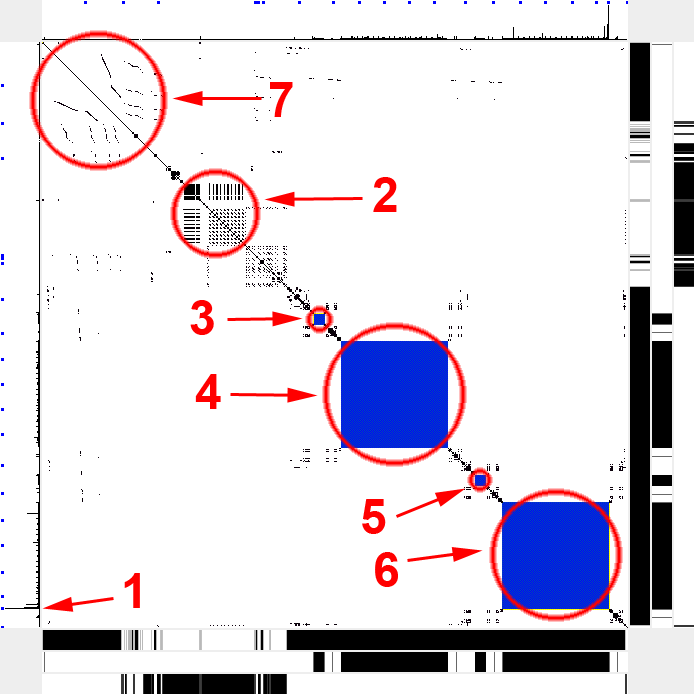
\includegraphics[width=0.5\textwidth]{lviz/cp-xcopy.png}
\caption{Self-comparison event-ordered VDP of {\tt xcopy}
copying 8 files of different sizes with the following configuration rules:
}
\begin{tabular}{ll}
DP match : & operation + parameter (pathname)\\
DP color : & magenta $\rightarrow$ source; cyan $\rightarrow$ destination;\\
 & black $\rightarrow$ other\\
Bar1 color : & black $\rightarrow$ file operation\\
Bar2 color : & black $\rightarrow$ source/destination files\\
Bar3 color : & black $\rightarrow$ registry operation
\end{tabular}
\label{fig:cp-xcopy}
\end{center}
\end{figure}


% \TODO{reviewer 2:
% Move figure 4 closer to the text where it is explained (section 3.3) Actually
% this section is hardly informative. It uses a lot of forward references so I
% have to jump all across the paper to see what it really tries to say. I think
% this section could be skipped since it does not bring additional value in the
% discussion at this point.
% }

Figure~\ref{fig:cp-xcopy} illustrates the event-ordered VDP
of a trace of running
{\tt xcopy} to copy two directories with files of different sizes.
The VDP uses self-comparison of the {\tt xcopy} trace with
the DP matching rule on operation and parameter (resource pathname).
The VDP configuration consisting of a DP ordering, DP matching rule,
DP coloring rules and barcode coloring rules
is given in the caption of the figure.
The non-white regions inside the DP show when {\tt xcopy} is using the
same resource with the same operation and parameter.
Its color represents the resource.
Each blue square is the aggregated visualization effect from
copying a file (see Section~\ref{sec:cp}).
The file sizes are apparent from the sizes of the small (region 3 and 5)
and big (region 4 and 6) blue squares.
We can see that file operations are performed at the start (barcode 1),
but those files are neither source nor destination files (barcode 2).
Registry operations are performed relatively
quickly compared to file operations,
because the blue ticks in the histogram above region 2 are spaced further apart
than the blue ticks above region 4 and 6.
Further discussion on this example is in Section~\ref{sec:cp}.

The DP user interface allows exploration of the trace by zooming in
This allows us to see quite different detail from an aggregated view.
We can see the effects of visualizations at different scales,
Figure~\ref{fig:cp-xcopy} shows the aggregate behavior which
is a different picture from the magnified view in
Figure~\ref{fig:cp-zoom} which shows the individual file operations in {\tt xcopy}.
Zooming creates a new window as one may want to see many different
detail levels at the same time. Clicking inside the DP selects
a pixel to give more details of the events aggregated in that pixel. When
the mode is event-ordering, the events displayed are those events contained
in that pixel. Whereas with time-ordering or time-duration-ordering,
the events are those events which intersect in time with the time interval
represented by that pixel.

\begin{figure}[htb]
\begin{center}

\includegraphics[width=0.10\columnwidth]{lviz/cp-zoom.png}
\caption{The alternate zoomed-in view of a blue region in
Figure~\ref{fig:cp-xcopy} showing reading (magenta) and writing (cyan) operations.
}
\label{fig:cp-zoom}
\end{center}
\end{figure}

% {Zoom and Click}.
% Zoom is one of the most important features that we must have.
% The first time the DotPlot is created, it encompases the entire log files
% that may contain hundred of thousands events.
% The pixel shown in this state contains aggregated number of events
% and the color might be seen as the addition of multiple colors.
% Zoom allows us to go deep into a particular region of interest
% and explore the traces in a more fine grained manner.
% Clicking on the DotPlot area will print out the events
% residing in the clicked region which is very helpful in exploration process.
%
%
% We designed our DotPlots UI to implement the above control operations.
% We use an extensive configuration file to specify most of the parameters for the visualization
% and we use command line interface to interact with the UI.
% The static parameters in the configuration file includes:
% list of log files, list of color rules (regex / plain search pattern),
% DotPlot fields selection, DotPlot color rules, Barcode color rules,
% invert color option, gamma correction value, histogram equalization option, etc...

% The command line accepts 4 commands: "dpe" to render a DotPlot Event-Ordering,
% "dpt" is for DotPlot Time-Ordering, "dptd" is for DotPlot Time-Duration-Ordering,
% and "reload" to reload the configuration file.
%
% A UI frame will pop out when one of the "dpe", "dpt", "dptd" command is put.
% The UI looks like \TODO{Figure ?}
%

\subsection{VDP Implementation and Scalability}
\label{sec:lviz-imp}

There are two important challenges in implementing VDP in \code{lviz}.
Firstly, traces are usually much larger than the size of the screen.
The challenge is to be able to still have usable visualizations given that
there will not be sufficient pixels to show every event.
Secondly, rendering a VDP on large traces needs to be sufficiently fast to
meet interactive UI needs (i.e sub-second response).
Finally, our implementation takes advantage of parallelism given
the trend in multi-core processors.
In this section, we describe an effective and efficient implementation
which meets these challenges.

% Third, a ruler and barcode-like stripes for each axis of the DP
% are added to give additional insight about the region of the inner DP.
% as well as caching can help a lot in responsiveness.

% To fit $100K$ events in a small window screen, a pixel often has
% to accommodate more than one event which in turn will determine
% the brightness / intensity of the pixel.
% The intensity of a pixel is determined by how much
% events in that pixel is a match according to DP matching rule
% (ie. match by program name, path, etc...).
% The hash or message digest (ie. MD5) of the matched fields is
% used to speedup the process of matching tests.
% A pixel that has 10 matched events will look brighter than a pixel
% that has 3 matched events.
% This introduces a grayscale color extension to the DP.
% When the number of matched events are too big, sometimes it exceeds
% the threshold of a grayscale color range [0..255].
% To handle this case, we have $gamma$ normalization to adjust
% the brightness of the pixel. First, the intensity
% (the number of matched events) of each pixel is translated
% to a continuous range value between zero and one inclusive.
% Then each value is mapped to an equation $y = x^(1/g)$ where $g$ is the gamma value.
% The resulting value is then translated to a grayscale color range value [0..255].
% This allow us to reveal the low-intensity pixel.
% The difference can be seen in
% \TODO{Figure~\ref{xx} add explanation to the figures on the differences}.
% Another method to reveal the low intensity pixel is through
% histogram equalization \TODO{cite} which allows for areas with lower
% intensity to have a brighter display without affecting the global intensity.

\begin{figure}[tb]
\begin{center}
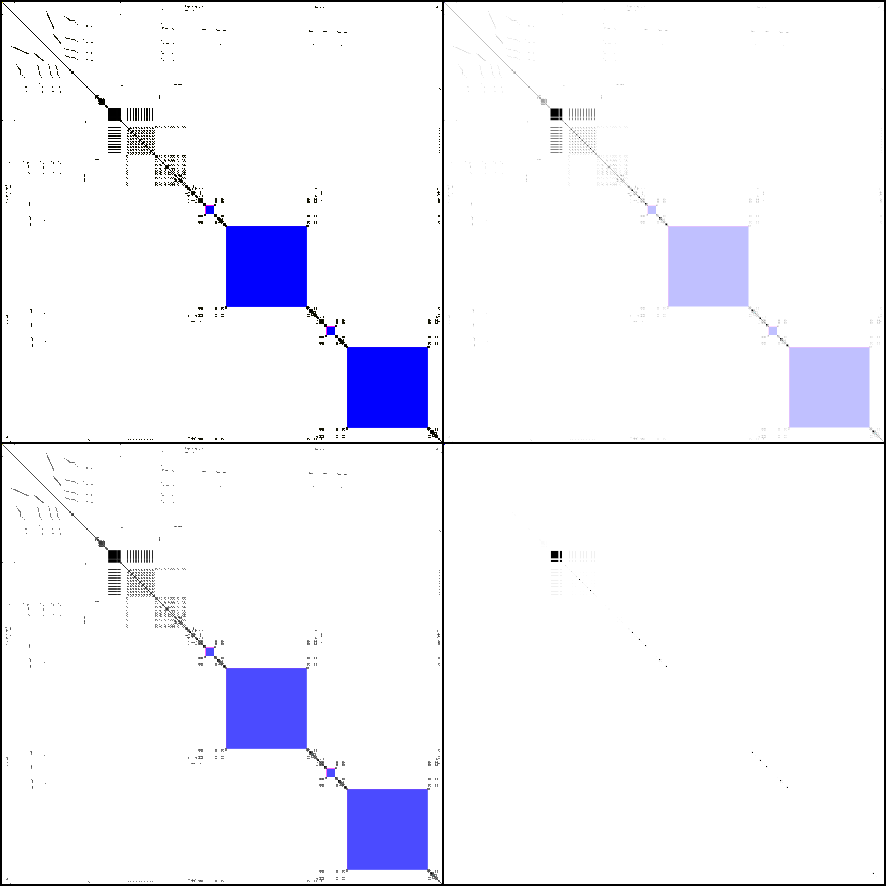
\includegraphics[width=0.5\textwidth]{lviz/gamma.png}
\caption{Clockwise from top-left:
histogram equalization, $\gamma=1$,
$\gamma=1/4$ and $\gamma=4$.
}
\label{fig:gamma}
\end{center}
\end{figure}

Consider a trace with $N$ events and
a display window size with width $W$ and height $H$.
For large traces, e.g. $N=10^6$, clearly $N \gg W$ and $N \gg H$,
and a binary DotPlot with two traces of $N=10^6$ corresponds to an
image with $10^{12}$ pixels (terrapixel).
Our VDP visualization aggregates multiple events into a single pixel,
normalizing it to RGB intensities between $0\ldots255$.
Unlike a digital photo, the intensity of a pixel could be up to $N$,
since aggregating events could end up with all of them
in a single pixel which could easily exceed 255.
\code{lviz} provides two options to deal with this issue by borrowing 
ideas from image processing.
The first is to simply normalize the values.
We extend normalization to include gamma correction, i.e. given an input value $x$,
the output value $y$ is mapped using the equation $y=x^{1/\gamma}$
(pure normalization corresponds to $\gamma = 1.0$).
The second option is histogram equalization which is
a well-known technique in image processing.

% \TODO{reviewer 3:
% The visual scalability discussion in section 4 opens up some serious questions.
% If I understand correctly, what is done is basically aggregation of colors like
% in image processing? This is very dangerous, since a visualization application
% should aggregate the actual data values, or more exactly even, the semantics of
% these values, and not the color mapped values. Just adding up or averaging
% colors can produce meaningless colors or even worse colors which exist in the
% used color map but have another meaning. See for example the work of D. Holten
% et al referred earlier or the work of T. Munzner on accordion drawing,
% guaranteed visibility, and the sequence juxtaposer comparison (available at
% http://www.cs.ubc.ca/~tmm/papers.html)
% }

Figure~\ref{fig:gamma} shows our {\tt xcopy} example visualized
with various normalization options.
In this example with an event-ordered VDP,
the intensity of a pixel shows how many matching events there are in the DP.
We see that histogram equalization (the default) is usually effective
in allowing matching burst events (high intensity) to seen together
with spread out events (low intensity).
While smaller $\gamma$ shows details of the high intensity events,
larger $\gamma$ shows low intensity events.

Most of the cost of rendering a VDP has to do with various forms of
matching: applying DP matching, DP coloring and barcode rules.
We can optimize the rendering to reduce matching costs by pre-processing
the traces. \code{lviz} performs the pre-processing steps when reading the
traces. Subsequent visualizations such as zooming in then make use of
the pre-computed results of the pre-processing phase.

An event in the raw trace is simply a string.
The pre-processing steps involves reducing an event to
a digest value as a more compact representation for DP matching
to operate on and also pre-computing the
results of various coloring rules.
Each event is represented as a hash value which we call a {\em digest}.
The digest helps to speed up event comparisons
as comparing digest values of events is much faster than
the corresponding string comparison, e.g. string matching is slow
as the strings of an event property often have a long common prefix such
as absolute pathname.
The digest of an event is computed based on the DP matching rule that specifies
how to tell if events are considered similar (Section~\ref{sec:lviz-vis}).
For example, if the matching rule is 
{\em program name + operation type + resource name}, the digest
of the event is a hash on those three properties of the event in that order.
We will refer to all the events having the same digest under
the set of DP matching rules as a {\em digest group}.
Thus, the number of digest groups in a trace is equal to the number of distinct hash values.
Note that an event can only belong to one digest group and the hash function
should be good enough to be effectively collision free so that 
two events which do not match (according to the DP matching rule) are
not hashed to the same digest group.

% The DP coloring rules extend the visualization to 24-bit color DP.
% We employ a pre-processing strategy 
% to speedup the matching of color rules (DP and Barcode).
% Once two events are considered a match by the DP matching rule, 
% those events will be colored based on the DP color rules.
It is common that the pattern in a coloring rule only needs a string
match.
Since there can be many color rules, we want to avoid applying
to the matching events one rule at a time.
We instead employ the Aho-Corasick's string matching
algorithm \cite{aho1975efficient}
to compile all the rules (the string patterns) into a single automaton.
This allows us to identify the color in a single pass
rather than multiple passes for each rule.

\begin{algorithm}[htb]
\KwIn{$L_X[0\ldots N-1]$ as log X; and $L_Y[0\ldots N-1]$ as log Y}
\KwOut{2D array $S[0\ldots W-1,0\ldots H-1]$ as pixel intensity}
\BlankLine
zero fill $S$\;
\For{$x\leftarrow 0$ \KwTo $N-1$}{
  \For{$y\leftarrow 0$ \KwTo $N-1$}{
    \If(\tcp*[f]{based on DP matching rule}){$L_X[x]$ matches $L_Y[y]$}{
      $S[xW/N,yH/N] ++$
    }
  }
}
\caption{Naive $O(N^2)$ Algorithm}
\label{alg:lviz-naive}
\end{algorithm}

The two pre-processing steps above are performed once and
cached in memory for later use when rendering the VDP.
The VDP rendering has to be fast as it is
used interactively for real-time browsing 
which entails zooming in on a region within the DP.
As the number of events in a trace, $N$, grows in order of hundreds of thousands,
the naive DP Algorithm~\ref{alg:lviz-naive}
takes $O(N^2)$ becomes infeasible.
To simplify our illustration, we assume both logs have the same number
of events.
We developed a new DP rendering algorithm which scales well to large traces.

\begin{algorithm}[htb]
\KwIn{$L_X[0\ldots N-1]$ as log X; and $L_Y[0\ldots N-1]$ as log Y}
\KwOut{Associative array $D_X[d]$ whose key $d$ is the digest of an event
and value is a set of integers representing indexes of events in $L_X$ whose
digests are $d$. Similarly for $D_Y[d]$.}
\BlankLine
\For{$x\leftarrow 0$ \KwTo $N-1$}{
  $d\leftarrow digest(L_X[x])$ \tcc*[l]{digest() calculates the digest based on the DP matching rule}
  insert x to the set $D_X[d]$
}
\For{$y\leftarrow 0$ \KwTo $N-1$}{
  $d\leftarrow digest(L_Y[y])$\;
  insert y to the set $D_Y[d]$
}
\caption{Preprocessing step to get digest group}
\label{alg:lviz-algpre}
\end{algorithm}

\begin{algorithm}[htb]
\KwIn{$D_X[d]$ and $D_Y[d]$ from Algorithm~\ref{alg:lviz-algpre}}
\KwOut{2D array $S[0\ldots W-1,0\ldots H-1]$ as pixel intensity}
\BlankLine
zero fill $S$\;
\ForEach{digest $d$}{
  \ForEach{$x$ in $D_X[d]$}{
    \ForEach{$y$ in $D_Y[d]$}{
      $S[xW/N,yH/N] ++$
    }
  }
}
\caption{New algorithm for large screen size}
\label{alg:lviz-alg1}
\end{algorithm}

The core of new DP rendering algorithm is based on two observations.
The first observation is that for each matching event,
a certain intensity value can be added incrementally.
Two events are considered a match if they are in the same digest group.
Events in different digest groups will never match thus will never be rendered.
The incremental algorithm effectively processes only the events
that contribute to the visualization and prunes all other events.
Consider digest group $D_i$ which has $S_i$ events.
It can be processed in time $O(S_i^2)$
and the result for this digest group can be added incrementally to the 
end result.
This significantly reduces the number of matching comparisons needed
from $O(N^2)$ down to $\sum_{i=1}^{G} S_i^2$
where $G$ is the number of digest groups in the trace.
Algorithm~\ref{alg:lviz-algpre} pre-process the two logs $L_X$ and $L_Y$
into digest groups stored in associative arrays $D_X$ and $D_Y$.
This preprocessing step takes $O(N)$ time and is executed only once.
Algorithm~\ref{alg:lviz-alg1} iterates each digest group and accumulates
the number of matches.

\begin{algorithm}[htb]
\KwIn{$D_X[d]$ and $D_Y[d]$ from Algorithm~\ref{alg:lviz-algpre}}
\KwOut{2D array $S[0\ldots W-1,0\ldots H-1]$ as pixel intensity}
\BlankLine
zero fill $S$\;
\ForEach{digest $d$}{
  declare temporary integer array $S_X[0\ldots W-1]$ and $S_Y[0\ldots H-1]$\;
  zero fill $S_X$ and $S_Y$\;
  \lForEach{$x$ in $D_X[d]$}{
    $S_X[xW/N] ++$
  }\;
  \lForEach{$y$ in $D_Y[d]$}{
    $S_Y[yH/N] ++$
  }\;
  \For{$w\leftarrow 0$ \KwTo $W-1$}{
    \For{$h\leftarrow 0$ \KwTo $H-1$}{
      $S[w,h]\leftarrow S[w,h]+S_X[w]\times S_Y[h]$
    }
  }
}
\caption{New algorithm for small screen size}
\label{alg:lviz-alg2}
\end{algorithm}

However, in the worst case, a digest group $S_i$ can be as large as $N$.
This drawback leads us to the second observation which
gives an optimization for the case when the digest group size is large.
It exploits the fact that $N > W\times H$ and often also $N \gg W\times H$.
Consider a digest group with $S_i$ events.
The intensity (color) for each event in that group can be recorded as
its projection on the X and Y axis of the window.
This is easily done by keeping track of the color intensities in
two arrays with size $W$ and $H$ respectively in $O(S_i)$ time.
Therefore, the resulting DP on a window of size $W \times H$
can be drawn based on the projected intensities in $O(S_i + W\times H)$ time,
as shown in Algorithm~\ref{alg:lviz-alg2}.

\begin{algorithm}[htb]
\KwIn{$D_X[d]$ and $D_Y[d]$ from Algorithm~\ref{alg:lviz-algpre}}
\KwOut{2D array $S[0\ldots W-1,0\ldots H-1]$ as pixel intensity}
\BlankLine
zero fill $S$\;
\ForEach{digest $d$}{
  \nlset{$\alpha$} \eIf{$|D_X[d]|\times |D_Y[d]|<|D_X[d]|+|D_Y[d]|+W\times H$}{
    \ForEach{$x$ in $D_X[d]$}{
      \ForEach{$y$ in $D_Y[d]$}{
        $S[xW/N,yH/N] ++$
      }
    }
  }{
    declare temporary integer array $S_X[0\ldots W-1]$ and $S_Y[0\ldots H-1]$\;
    zero fill $S_X$ and $S_Y$\;
    \lForEach{$x$ in $D_X[d]$}{
      $S_X[xW/N] ++$
    }\;
    \lForEach{$y$ in $D_Y[d]$}{
      $S_Y[yH/N] ++$
    }\;
    \For{$x\leftarrow 0$ \KwTo $W-1$}{
      \For{$y\leftarrow 0$ \KwTo $H-1$}{
        $S[x,y]\leftarrow S[x,y]+S_X[x]\times S_Y[y]$
      }
    }
  }
}
\caption{Combined algorithm from \ref{alg:lviz-alg1} and \ref{alg:lviz-alg2}.
(Line $\alpha$ can be further tuned with some constant factors)}
\label{alg:lviz-alg3}
\end{algorithm}

Both algorithms can be combined together to
get the best of both worlds, which gives
a DP rendering time complexity of $\sum_{i=1}^{G} min(S_i^2, S_i + W\times H)$,
as shown in Algorithm~\ref{alg:lviz-alg3}.
That is, for each digest group $S_i$ that satisfies $S_i^2 < S_i+W\times H$, 
the $O(S_i^2)$ algorithm is used;
otherwise, the $O(S_i + W\times H)$ algorithm is used to obtain a sub-image.
Adding the intensities of all the sub-images of all digest groups gives the final image.

We illustrate the complexity of the algorithm to process $N=10^6$ events.
The worst case is when the number of digest groups $G$ is $10^3$
and each digest group has size $10^3$.
Suppose the window screen size is $1000\times 1000$.
Then the first $O(S^2)$ algorithm is used giving $GS^2 = 10^9$ operations.
If the window size is resized to $600\times 400$, then
the second $O(S+W\times H)$ algorithm is used giving $G(S+WH)=2.41\times 10^8$ operations.
This is much faster than the naive algorithm which would take $O(10^{12})$
operations.
The best case is achieved when each digest group only contains one event.
This means $G = 10^6$ and the number of operations
is $G S^2=10^6$.
Another good case is when there is only one digest group,
so $S=10^6$ and the number of operations is $G(S + W\times H)=1.24\times10^6$.

\code{lviz} is multi-threaded to make use of multi-core processors.
The pre-processing steps and rendering algorithms can be easily parallelized.
The events in the trace can be split up into several sub-traces and 
the pre-processing can be applied to each sub-trace
independently and in parallel.
We implemented and tested the rendering algorithm using
OpenJDK 1.6.0\_18 (64bit) on an Intel Core i7-960 3.20GHz
machine with 12G RAM.
An uncompressed 120MB trace file with 558K events took 2.8 seconds
to read and finish the two pre-processing steps using 8 threads.
To see the effectiveness of parallel pre-processing, it took 6.0 seconds,
when the execution is single-threaded.
In our rendering algorithm, each digest group can be processed
independently and in parallel as there is no dependency between digest groups.
We also render all the sub-components
of a VDP, the DP, barcodes, and histograms in parallel.
It took about 0.5 seconds to render the trace where the DP has 550K events
on both axis.
Thus, \code{lviz} can process large traces with sufficient real-time response
when the user interactively zooms/resizes the VDP or changes the histogram.

To speed up subsequent runs, \code{lviz} creates a cache containing the results
of the pre-computations of the digest, DP color, barcodes color
of each event since they require the most computation
and are the bottleneck of the system. The cache avoids recalculating the
digest and the coloring rules every time the program is run.
This cache is rebuilt if the corresponding rules change.
Loading from the cache skips the pre-computation steps and
cuts down the trace loading time to 1.3 seconds.
The speedup is more significant when the matching and coloring rules are
more complicated.

% \TODO{reviewer 2:
% The scalability solution seems, from what I can read, well thought. However I
% wonder if a comparatively fast result, if not a faster one, could not have been
% obtained, with less programming effort, by using a pixel shaders or CUDA
% implementation.
% }

% While the DP treats each event independently,
% RTG has to show the connections
% between events for visualizing the resource life cycle.
% If we consider each event as an operation on a resource
% (e.g. file or registry key),
% each resource is associated with a sequence of operations which includes
% creating a new one, opening an existing one, reading, writing/modifying, closing, deletion.
% If we further assume the resource life cycle has three states:
% non-existence, exists but not
% opened, opened, we can use the sequence of operations to
% reconstruct the state transitions for RTG visualization.
% However, there are some exceptions to be noted.
% Firstly, we may be dealing with a trace
% only during some time period, i.e. some
% resource can be opened before logging happens,
% thus we have to ``guess'' the initial state of the resource.
% We employ a heuristic based on the first observed operation of each resource.
% Secondly, file deletion in Windows is done in a special system call
% {\tt NtSetInformationFile} which puts file into ``delete after close'' state.
% In order to delete a file, one should first open the file,
% then call {\tt NtSetInformationFile} to set the ``delete after close'' state,
% finally close the file and if no other processes are opening the file, it will
% be deleted.
% Lastly, there is an additional rename operation
% which is translated in our RTG as a combination
% of deletion and creation operations.

\section{Case Studies}
\label{sec:study}

The following case studies show how \lviz{} can be used to
understand system behavior and to solve system or application problems.
We first use a well understood task, file copying,
to familiarise the reader with \VDP{}.
We then use a software compilation example to show how \VDP{} can
be used for software failure diagnosis.
We use two visualizations on whole system traces to understand
how the operating system works and examine performance problems.
Lastly, we use \VDP{} to examine performance problems in a browser benchmark.
These examples also illustrate that the \VDP{} visualization is highly
customizable and in practice, one could use many different visualizations
on the same trace.

% In order to demonstrate the potential and power of visualizing system traces,
% we have developed a visualization tool \VDP{} using an extension of
% dotplots \cite{dnadp}.
% Dotplots were used to show sequence similarity in
% DNA \cite{dnadp} and music \cite{audio}.
% Our \VDP{} dotplots (or simply \VDP{} for both the visualization and tool)
% extends the basic dotplot to get a flexible visualization
% which can be tailored to visualize different kinds of behavior.
% Furthermore, \VDP{} uses a number of novel extensions geared towards
% understanding software behavior whereas traditional uses of dotplots
% are for showing sequence similarity.

The notation Bar $n$ refers to the $n$th barcode.
The configuration of each visualization is described in the corresponding
figure caption.

\subsubsection{Comparing File Copying Programs}
\label{sec:cp}

% \TODO{problems to solve: 1. finding repeated patterns
% 2. diagnose performance problem (8k buffer)}

% \begin{figure}[htb]
% \begin{center}
% 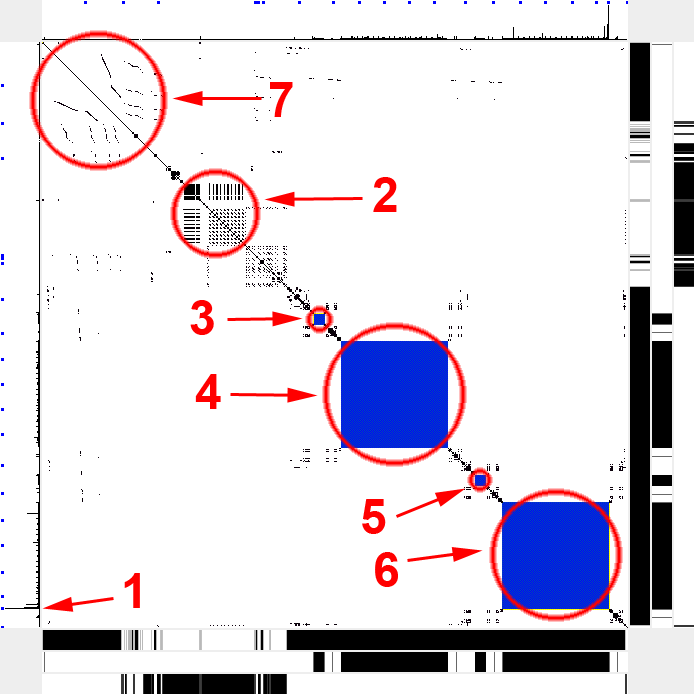
\includegraphics[width=1.0\columnwidth]{lviz/cp-xcopy.png}
% \caption{Self-comparison event-ordered \VDP{} of {\tt xcopy}
% copying 8 files of different sizes with the following configuration rules: 
% }
% \begin{tabular}{ll}
% DP match : & operation + parameter (pathname)\\
% DP color : & magenta $\rightarrow$ source; cyan $\rightarrow$ destination;\\
%  & black $\rightarrow$ other\\
% Bar1 color : & black $\rightarrow$ file operation\\
% Bar2 color : & black $\rightarrow$ source/destination files\\
% Bar3 color : & black $\rightarrow$ registry operation
% \end{tabular}
% \label{fig:cp-xcopy}
% \end{center}
% \end{figure}

\begin{figure}[htb]
\begin{center}

\includegraphics[width=0.10\columnwidth]{lviz/cp-zoom.png}
\caption{The alternate zoomed-in view of a blue region in
Fig.~\ref{fig:cp-xcopy} showing reading (magenta) and writing (cyan) operations.
}
\label{fig:cp-zoom}
\end{center}
\end{figure}

We use an example of a simple program and operation,
namely, file copying using \xcopy{}, to explain various
aspects of the \VDP{} visualization.
Fig.~\ref{fig:cp-xcopy} shows a self-comparison event-ordered \VDP{} of
\xcopy{} copying 8 files with sizes
1MB, 10KB, 10MB, 100KB, 1MB, 10KB, 10MB and 100KB and in that given order.
A self-comparison \VDP{} has a 45$^\circ$ diagonal line from top-left to 
bottom-right corner because events on the diagonal always match.
The structure of the files being copied is visible as blue squares in
Region {\em 3}, {\em 4}, {\em 5} and {\em 6} which show copying the
first 1MB and 10MB, then the second 1MB and 10MB files.
It is interesting to see the effect of scale on the visualization.
At this scale, which shows everything, the relative file sizes are also
visible for the large files.  The smaller 10KB and 100KB files are 
too small to be seen at this scale but are visible when zoomed in.
By correlating Bar1 and Bar2,
we find that there are some file related operations in the early phase,
but those files are neither source nor destination files of \xcopy{}.
This might seem surprising. To answer that question, we
click on Region 7, which shows that
the files in question are DLLs. Thus, the top-left region 
shows \xcopy{} loading DLLs.

Bar3 shows that Region {\em 2} has many registry operations which might
be surprising for a file copying task.
% This shows that a command line program can also have many
% registry operations.
The histogram spike at Region 1 shows that some events at the end of the
trace take a long time.
Fig.~\ref{fig:cp-zoom} is a zoomed-in view to one of the blue squares in
Fig.~\ref{fig:cp-xcopy}.
The checkerboard-like pattern shows alternating read (magenta) and write
(cyan) operations which is what we expect for file copy.
Since $cyan+magenta=blue$,
this explains that the blue squares in Fig.~\ref{fig:cp-xcopy} represents
reading from source files and writing to destination files.
We see also that visualizations at different scales can be used for
different purposes.
The extreme magnification in Fig.~\ref{fig:cp-zoom}
shows the actual operations but may be too detailed a view for
the overall picture which emerges at the other extreme in 
Fig.~\ref{fig:cp-xcopy}.

\begin{figure}[tbh]
\begin{center}
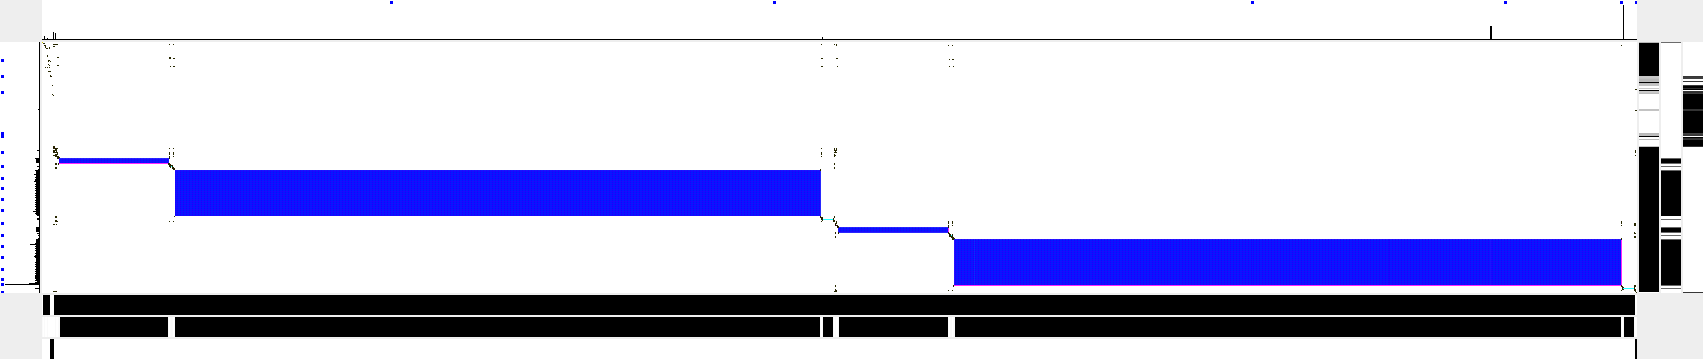
\includegraphics[width=1.0\columnwidth]{lviz/cp-xvc.png}
\caption{Event-ordered \VDP{} comparing {\tt cp} (x-axis) and {\tt xcopy} (y-axis) copying
the same files. 
The configurations are the same as in Fig.~\ref{fig:cp-xcopy}.
}
\label{fig:cp-xvc}
\end{center}
\end{figure}
%
\begin{figure}[htb]
\begin{center}
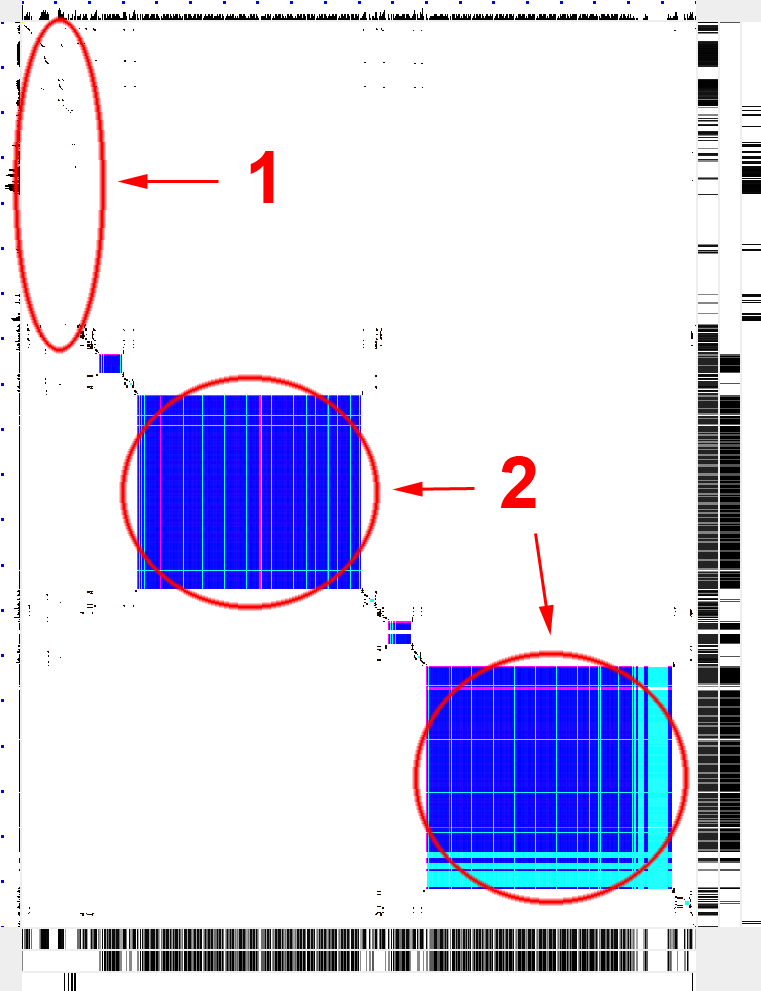
\includegraphics[width=0.6\columnwidth]{lviz/cp-64k.png}
\caption{Time-ordered \VDP{} comparing {\tt cp-64k} (x-axis)
and {\tt xcopy} (y-axis).
The configurations are the same as in Fig.~\ref{fig:cp-xcopy}.
}
\label{fig:cp-64k}
\end{center}
\end{figure}

In general, a \VDP{} is used with two traces rather than a single
trace as in a self-\VDP{}.
% Fig. \ref{fig:cp-xcopy} shows a \VDP{} which compares of a {\tt xcopy}
% trace against itself, i.e. a self-similarity comparison.
% Two different traces can also be compared with one trace on the X axis
% and the other trace on the y-axis.
Fig.~\ref{fig:cp-xvc} compares {\tt cp} (x-axis: a Windows version
of GNU {\tt cp}) and {\tt xcopy} (y-axis) copying the same 8 files.
% {\tt cp} is the Windows version of the file copying program included
% in GNU coreutils.
The \VDP{} is much wider than its height, giving
wide blue rectangles instead of blue squares 
(Fig.~\ref{fig:cp-xvc} versus Fig.~\ref{fig:cp-xcopy}).
% \TODO{double check width:height, shouldnt it be 16x?}
% Measuring the width and height of the rectangle,
% we find the ratio of width to height is approximately ? times.
Thus, {\tt cp} performs many more operations than {\tt xcopy}.
To investigate further, zooming in and examining individual events, 
we find that each read and write operation uses a buffer size of 4K,
while {\tt xcopy} uses 64K.
This means that {\tt cp} has 16 times more read and write operations
than {\tt xcopy}.
This is consistent with the width-height ratio in the visualization.

% \begin{figure}[htb]
% \begin{center}
% \includegraphics[width=1.0\columnwidth]{cp-xvct.png}
% \caption{Same as Fig.~\ref{fig:cp-xvc} but the axises are in time units.}
% \label{fig:cp-xvct}
% \end{center}
% \end{figure}

In order to compare the performance of {\tt cp} and {\tt xcopy},
we can use a time-ordered \VDP{}.
% In time based \VDP{}, events are distributed on the axises based on their
% relative time to the first event, while in event based \VDP{}
% events are distributed uniformaly.
Changing the visualization to a time-ordered one (not shown)
shows that {\tt cp} runs slower than {\tt xcopy} though less than 16x.
We then modified {\tt cp} to obtain another version
{\tt cp-64k} which uses 64K buffers.
Fig.~\ref{fig:cp-64k} shows the time-ordered \VDP{} comparing
{\tt cp-64k} (x-axis) and {\tt xcopy} (y-axis).
From Region {\em 2}, we can see that copying of the largest file
is performed in about the same time in both programs.
However, {\tt xcopy} has a slow initialization 
(as shown in Fig.~\ref{fig:cp-64k} Region {\em 1} which includes the registry
operations in Fig.~\ref{fig:cp-xcopy} Region {\em 2}),
which causes {\tt xcopy} to be slower in total than {\tt cp-64k}.

% \TODO{discuss flexible configuration and exploration process also shown
% in the other case studies}



\subsubsection{A Software Build Case Study}
\label{sec:build}

\begin{figure}[htb]
\begin{center}
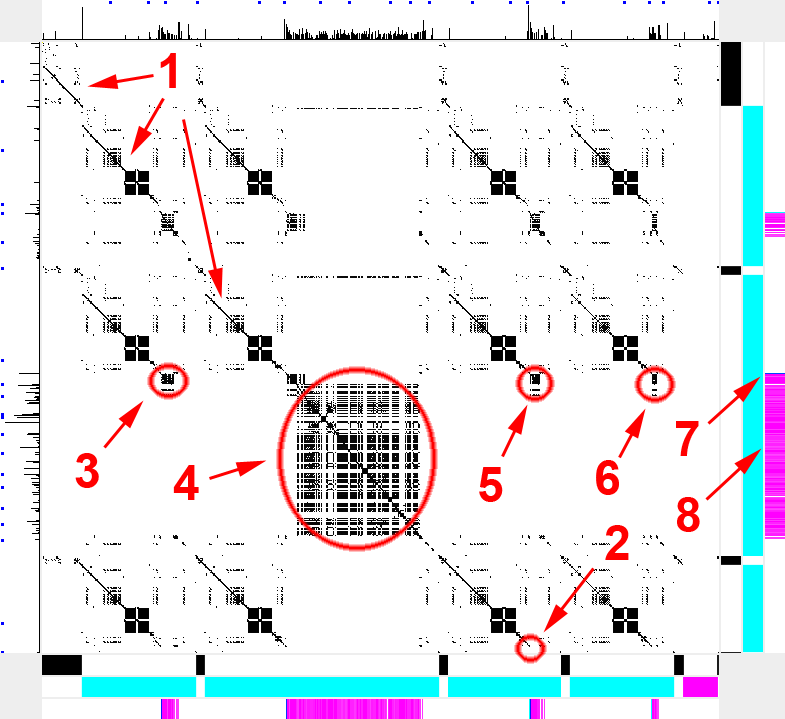
\includegraphics[width=1.0\columnwidth]{lviz/make-fail.png}
\caption{Event-ordered \VDP{} comparing a successful (x-axis)
software build process and a failed (y-axis) one.
%DP matching: program, operation and value (pathname);
%DP color: any=black;
%Bar1: {\tt nmake.exe}=black;
%Bar2: {\tt cl.exe}=cyan, {\tt link.exe}=magenta;
%Bar3: reading {\tt .c}/{\tt .h} files = cyan/magenta.
\label{fig:make-fail}
}
\begin{tabular}{ll}
DP match : & program + operation + value (pathname)\\
DP color : & black $\rightarrow$ any\\
Bar1 color : & black $\rightarrow$ {\tt nmake.exe}\\
Bar2 color : & cyan $\rightarrow$ {\tt cl.exe}; magenta $\rightarrow$ {\tt link.exe}\\
Bar3 color : & cyan $\rightarrow$ reading {\tt .c} files;\\
 & magenta $\rightarrow$ reading {\tt .h} files
\end{tabular}
\end{center}
\end{figure}

\begin{figure*}[htb]
\begin{center}
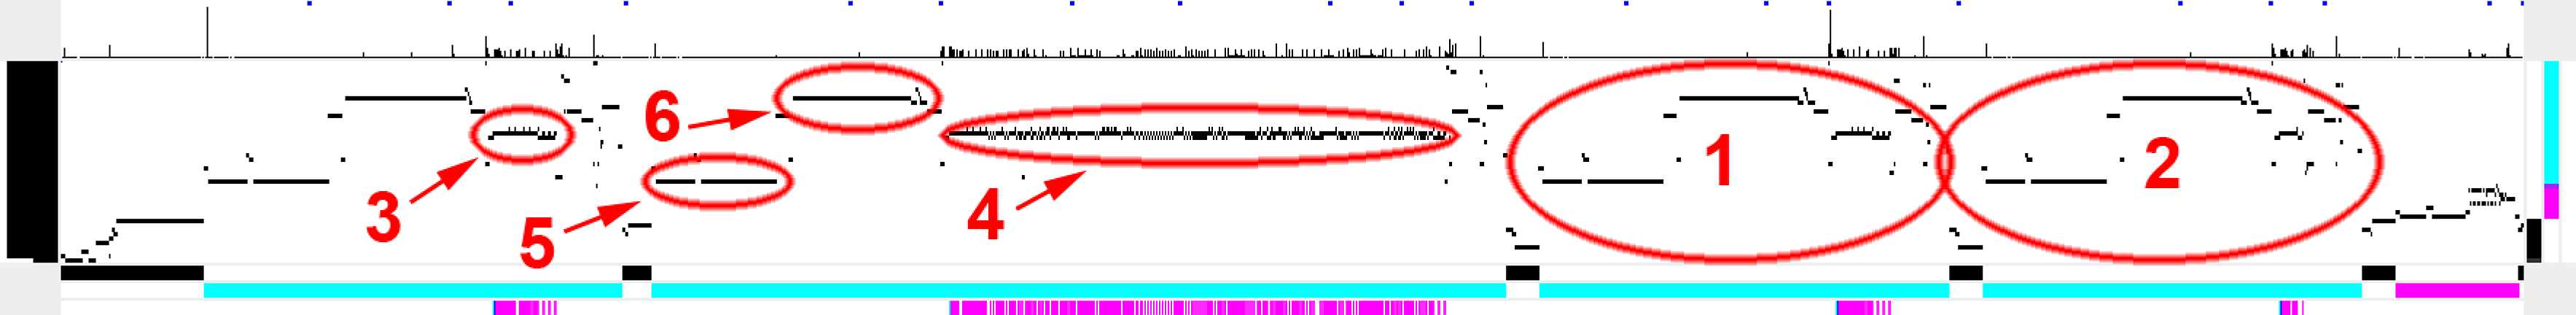
\includegraphics[width=1.0\textwidth]{lviz/make-pp.png}
\caption{Program point event-ordered \VDP{} of project build: pseudo program point trace (y-axis).
}
DP match: program name + program point;
DP color: black $\rightarrow$ any;
Barcode coloring rules are the same as in Fig.~\ref{fig:make-fail};
Bar3 in y-axis is undefined as the pseudo trace does not have operation type.
\label{fig:make-pp}
\end{center}
\end{figure*}

We now apply visualization to diagnose program failure.
In Fig.~\ref{fig:make-fail}, we compare a successful software project build
with a failed one to explain the failure.
The project consists of 4 C files, a header file and a {\tt makefile}.
We use {\tt nmake.exe} from Visual Studio to build the project.
To deliberately cause failure, one of the C files is changed
to be unreadable.

% Before identifying the cause of the failure,
We first explain what the visualization shows.
From the Bar2 of x-axis, 
we can see 4 {\tt cl.exe} processes (4 cyan regions), which tallies
with the number of C files.
There is one invocation of {\tt link.exe} (magenta),
occurring at the end of the trace.
By correlating Bar2 and Bar3, we see that
{\tt cl.exe} processes first read a C file (tiny blue bar in region {\em 7})
and then read a number of header files (long magenta bar in region {\em 8}).
Different {\tt cl.exe} processes read a different number of header files,
see sizes of regions {\em 3}, {\em 4}, {\em 5}, {\em 6} differ.

In a self-comparison \VDP{}, there will be a 45$^\circ$
diagonal line from top-left to bottom-right corner.
% The diagonal line means that the events
% on both x-axis and y-axis match (which is obviously true for self-comparison).
Fig.~\ref{fig:make-fail} shows a 45$^\circ$ diagonal (Label {\em 1})
with some breaks, from
the start to region {\em 2}, near the end of the failed build (y-axis).
It shows that the traces are basically similar till the failure point
when the build terminates.
By zooming in (not shown),
we see that the failure occurs at the third invocation of
{\tt cl.exe}, just before reading the C file.
Thus, the \VDP{} shows how file I/O works in the build and we use this
to identify a failed build.
One might argue that the compiler's error message is a better solution.
However, firstly,
not all software give detailed error message like the compiler in this case.
Secondly, due to software bugs, the error message could be wrong, while 
the system trace reports the actual underlying issues.

The build example is reused to show a visualization of the code structure
of {\tt cl.exe} in Fig.~\ref{fig:make-pp}.
We use a pseudo trace (y-axis) consisting of the program name
concatenated with its program point in the binary (an instruction address)
which is sorted by program name and address.
The program point comes from the stack walk corresponding to the event
and corresponds to the latest return address in the stack trace
coming from the executable or earliest DLL.
The x-axis trace is as before in Fig.~\ref{fig:make-fail}.

Region {\em 1} and {\em 2} show two invocations of {\tt cl.exe}
having similar patterns.
In fact, all 4 invocations follow the same pattern which can be broken
up into three main components:
region {\em 5}, {\em 6} and {\em 4}.
By zooming in and looking at the events, we infer that
region {\em 5} and {\em 6} is in the initialization phase of the compiler, which include
loading of DLL files and reading configurations from the registry.
Region {\em 6} is the reading of a large DLL {\tt rsaenh.dll}.
By looking at Bar3,
region {\em 3} and {\em 4} are the reading of C and header files.
As different C files have different header includes,
region {\em 3} and {\em 4} have different widths.
The fine squiggles in region {\em 3} and {\em 4} represent
three different file operations: open, read and close.
For each header file, there is one file open and close event,
with a differing number of file read operations depending
on the file size.
This makes the squiggles irregular.
Since this \VDP{} is based on program points, it shows directly the 
structure of the function calls. Thus, it visualizes
the code while Fig.~\ref{fig:make-fail} compares the operations
due to system calls.
It is also different from the source code visualization in \cite{tralfamadore}
and we do not need to rely on availability of source code.

The configurations play an important role in a \VDP{}.
Fig.~\ref{fig:make-matching} shows two \VDPs{} 
which are visually different from each other and also Fig.~\ref{fig:make-fail}
but they are all visualizations of the same underlying trace.
The \VDPs{} in Fig.~\ref{fig:make-matching} and 
Fig.~\ref{fig:make-fail} only differ in the DP matching rule and
the rest of the configuration is the same.
% The rest of the configuration and the two traces are exactly the same.
The left side \VDP{} in Fig.~\ref{fig:make-matching} uses only the event 
operation as the DP matching rule.
It can be used to highlight same or different operations.
The right side \VDP{} uses the program name, and can be used to
show different programs used in the project build process.

\begin{figure}[htb]
\begin{center}
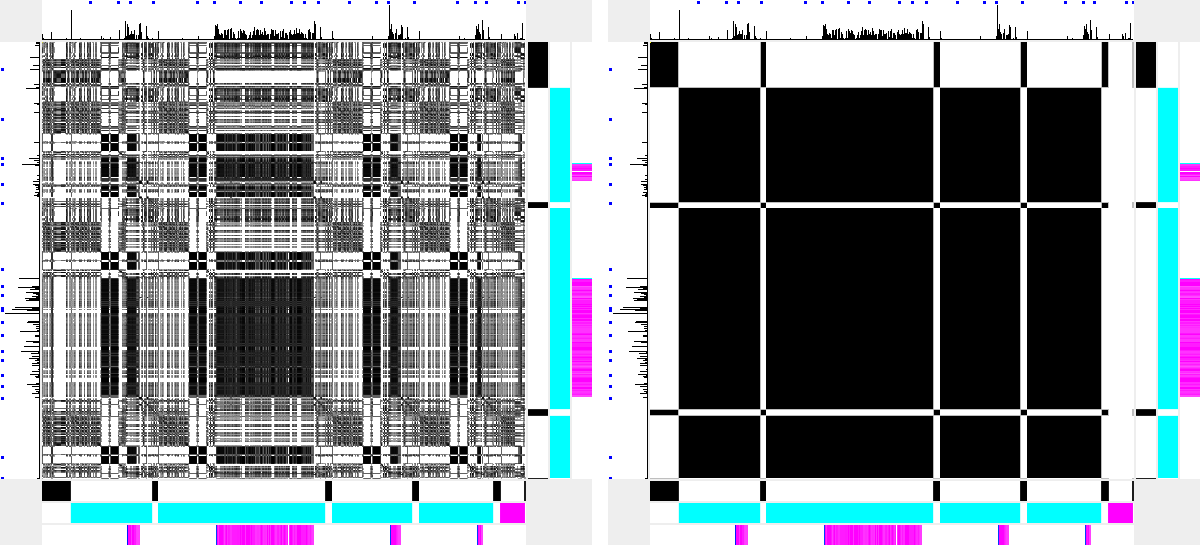
\includegraphics[width=1.0\columnwidth]{lviz/make-matching.png}
\caption{Changing the DP matching rule of Fig.~\ref{fig:make-fail}.
Left side DP matching rule is operation; Right side is program name.
}
\label{fig:make-matching}
\end{center}
\end{figure}

\TODO{reviewer 2:
In the second example, figure 8, a similar question: how do I know that a cyan bar is cl.exe and not some other
process - as a user I mean, not reading the legend of the figure? But the main question I have is why would a user go
to this level of effort to find why a build failed, he can always use the compiler's build log to find much more precisely
and more quickly what happened.
fixed.
}

\subsection{Visualizing Idle System Traces}
\label{sec:idle}

\begin{figure*}[htb]
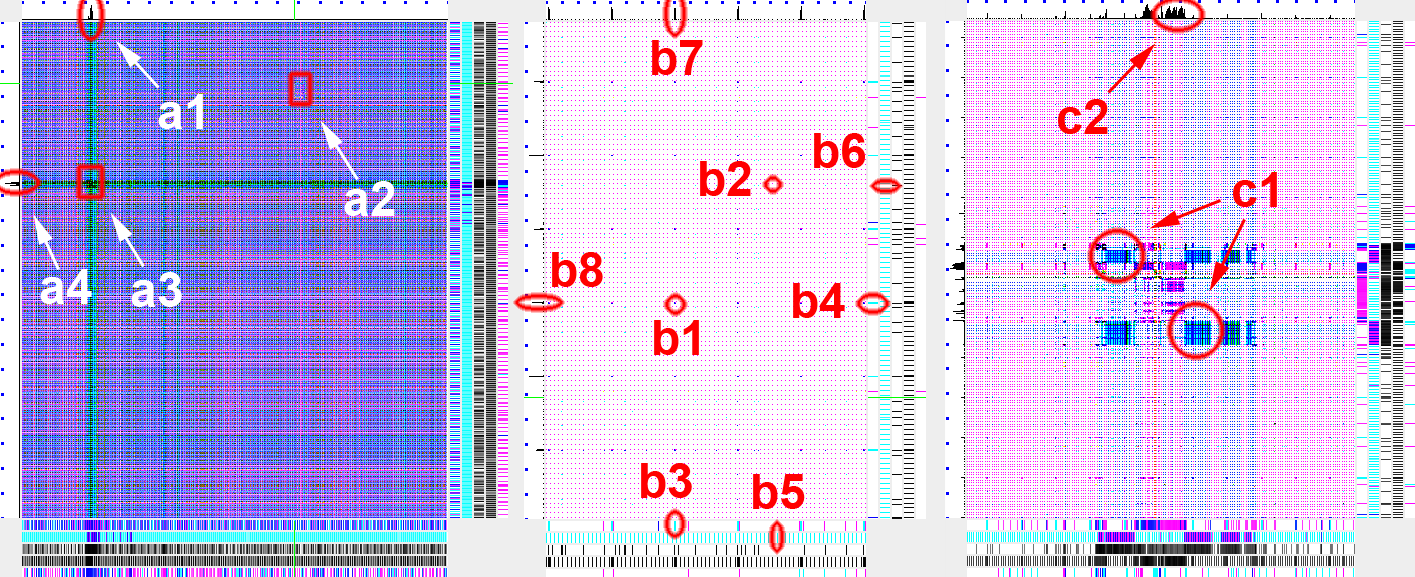
\includegraphics[width=1.0\textwidth]{lviz/idle-dp.png}
\caption{Time-ordered \VDP{} comparing two idle systems.
{\bf a.} (left) comparing one hour interval between two machines;
{\bf b.} (middle) zoom in of Region {\em a2};
{\bf c.} (right) zoom in of {\em a3}.
%DP Matching: (program,operation);
%DP color: file=cyan, registry=magenta, other operation=yellow;
%Bar1: lsass.exe=cyan, svchost.exe=magenta;
%Bar2: explorer.exe=cyan, wuauclt.exe=magenta;
%Bar3: file=black;
%Bar4: registry=black;
%Bar5: network=cyan, process\&thread creation\&termination=magenta.
The different DP color intensity in the zoomed views is caused by
histogram equalization.
}
\label{fig:idle-dp}
% \begin{tabular}{ll}
% DP match : & program + operation\\
% DP color : & cyan $\rightarrow$ file; magenta $\rightarrow$ registry; yellow $\rightarrow$ others\\
% Bar1 color : & cyan $\rightarrow$ lsass.exe; magenta $\rightarrow$ svchost.exe\\
% Bar2 color : & cyan $\rightarrow$ explorer.exe; magenta $\rightarrow$ wuauclt.exe\\
% Bar3 color : & black $\rightarrow$ file\\
% Bar4 color : & black $\rightarrow$ registry\\
% Bar5 color : & cyan $\rightarrow$ network, magenta $\rightarrow$ process \& thread creation \& termination
% \end{tabular}
{\it DP match}: program + operation;
{\it DP color}: cyan $\rightarrow$ file; magenta $\rightarrow$ registry; yellow $\rightarrow$ others;
{\it Bar1 color}: cyan $\rightarrow$ lsass.exe; magenta $\rightarrow$ svchost.exe;
{\it Bar2 color}: cyan $\rightarrow$ explorer.exe; magenta $\rightarrow$ wuauclt.exe;
{\it Bar3 color}: black $\rightarrow$ file;
{\it Bar4 color}: black $\rightarrow$ registry;
{\it Bar5 color}: cyan $\rightarrow$ network, magenta $\rightarrow$ process \& thread creation \& termination.
\end{figure*}


Previous examples compared the trace of particular programs
% against another
% so that we can compare the behavior of the two programs
(or to understand
how a program behaves using a self-similarity \VDP{}).
We now show that visualization can also be useful for system traces
as a whole -- a system trace is the complete trace of the entire operating
system for a period of time.

% \TODO{what is the problem}

When Windows is idle (i.e. no user interaction), 
system services and system processes still run.
We want to visualize whether such services and programs have 
(some expected) periodic behavior.
Fig.~\ref{fig:idle-dp}a (left) shows a time-ordered \VDP{} from two 
different idle machines for an hour at different times.
The size of the x and y-axis traces are 
851528 and 652713 events respectively.
% \footnote{
% Our \VDP{} tool handles large traces with real-time interaction.
% }
The configuration is described in the figure caption.
Bar1 and Bar2 show which events belong to
the four most active programs:
{\tt lsass.exe} is the Local Security Authority Subsystem Service which
enforces security;
{\tt svchost.exe} runs various services;
{\tt explorer.exe} is the graphical shell;
and {\tt wuauclt.exe} is windows auto-update service.
Bar3, Bar4 and Bar5 show the operation types.

Fig.~\ref{fig:idle-dp} shows periodic structure which appears
fractal-like.
Bar1 and Bar2 in Fig.~\ref{fig:idle-dp}a
show that events from {\tt lsass.exe}, {\tt svchost.exe} and {\tt explorer.exe}
occur continuously in the traces but {\tt wuauclt.exe} only occurs
during a short period of time.
Since this is time-ordering and the trace is one hour, we can conclude that
{\tt wuauclt.exe} occurs for about 7 minutes. (Bar2's magenta region
spans about 2
ticks in the histogram and there are 20 ticks in total.)
During this short period, we can see that a lot of events occur,
because the histogram at Region {\em a1} and {\em a4} have peaks.
We select two obvious regions to study the structure:
Region {\em a2} which is zoomed in Fig.~\ref{fig:idle-dp}b and 
Region {\em a3} zoomed in Fig.~\ref{fig:idle-dp}c.

We turn to the zoom in Fig.~\ref{fig:idle-dp}b.
Bar1 and Bar2 in
Fig.~\ref{fig:idle-dp}b show more clearly that
{\tt explorer.exe} (Region {\em b5} and {\em b6}) runs
more frequently than {\tt lsass.exe} (Region {\em b4} and {\em b3}).
Thus, we see two kinds of periodic events. The numerous dots such
as Region {\em b2} are the more frequent periodic events from 
{\tt explorer.exe} while the darker and less frequent dots such as
Region {\em b1} come from {\tt lsass.exe}.
Although {\tt explorer.exe} runs more frequently,
the event frequency histogram at Region {\em b7} and {\em b8} shows
that {\tt lsass.exe} has more events each time, hence Region {\em b1}
is darker than {\em b2}.
The white portions and together with the histogram show that there
are no other events in these portions of the idle trace.
% This means the load of {\tt explorer.exe} is spread out while
% the load of {\tt lsass.exe} is concentrated.

We have covered the periodic events in Fig.~\ref{fig:idle-dp}a except
for Region {\em a3}.
To explain Region {\em a3} and its zoom in Fig.~\ref{fig:idle-dp}c, 
we notice the cyan in Bar5 (network events) shows more activity.
Selecting those network events we find the
program is {\tt wuauclt.exe} (Windows update) --
both machines run Windows update at different time points explaining
the increase in network events.
% Selecting events in \VDP{} shows that the events are associated
% with {\tt wuauclt.exe} (Windows update) -- thus, it is Windows update
% running at a different point of time in both traces.
The dark Region {\em c1} shows that many of the events are the same 
in both machines in Windows update.
These events are file read and write to
{\tt C:\BS windows\BS softwaredistribution\BS datastore\BS datastore.edb}
(the Windows update database).
% We also see that network activity (outermost barcode) is higher in 
% Region {\em c3} during Windows update.
Other bursts of events in Region {\em c2} are generated by
{\tt svchost.exe} (it runs various Windows services) 
which operates on registry keys related to
windows installation.
% possibly due to the windows update.

This example shows that different machines not synchronized to 
each other have common periodic patterns and behavior.
We note that as we used idle traces, the frequency
of events will be low and a direct visualization is quite
faint. As such, \VDP{} employs equalization on the image 
to make the low frequency events more visible.

\TODO{reviewer 2:
In the example in 5.3, I understand that the task is to compare the behavior of Windows running idle on two different
machines. The question I have then is why would you use a 2D plot, when several histograms, stacked atop of each
other, could give you the same insight? That is, why is time ordering important here? I get the impression that the
same question holds for the system boot use case.
}

\subsection{System Boot}
\label{sec:boot}

\begin{figure*}[htb]
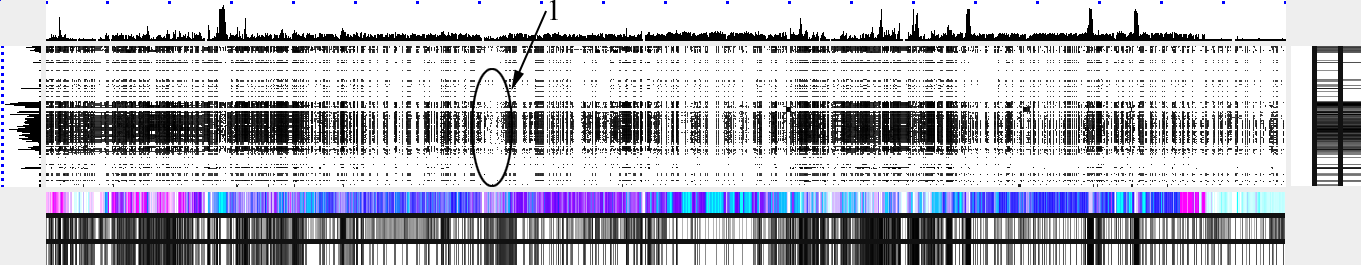
\includegraphics[width=1.0\textwidth]{lviz/boot-dp.png}
\caption{Time-ordered \VDP{} comparing boot
of a clean (Y axis) and a dirty (X axis) system.
}
\label{fig:boot-dp}
%\begin{tabular}{ll}
%DP match : & program + operation + parameter\\
%DP color : & black $\rightarrow$ any\\
%Bar1 color : & cyan $\rightarrow$ Google Desktop; magenta $\rightarrow$ AVG\\
%Bar2 color : & black $\rightarrow$ any program except Google Desktop and AVG\\
%Bar3 color : & black $\rightarrow$ file operation on Windows system directories\\
%\end{tabular}
{\it DP match}: program + operation + parameter;
{\it DP color}: black $\rightarrow$ any;
{\it Bar1 color}: cyan $\rightarrow$ Google Desktop; magenta $\rightarrow$ AVG;
{\it Bar2 color}: black $\rightarrow$ any program except Google Desktop and AVG;
{\it Bar3 color}: black $\rightarrow$ file operation on Windows system directories.
\end{figure*}

In Fig.~\ref{fig:boot-dp}, we use \lviz{} to investigate system boot and try to identify possible
factors causing a system to boot slowly.
To do this, we use a time-ordered \VDP{} to
compare a clean system which is known to boot quickly
with a (dirty) system which has many programs installed and boots slowly.

We see that the clean system boots much faster than the dirty system 
as the height is much shorter than the width.
Whenever Bar2 on the x-axis is not black,
the AVG (AVG antivirus) or Google Desktop is responsible for events.
We see that most of the events in the dirty boot are due to AVG or Google
Desktop.
We can also see from comparing Bar2 with Bar3
that the dirty system has other installed programs running
which are not in Windows directories.
%By looking at Bar1, we can clearly see that Google Desktop and AVG comprise about 5\% of boot time.

Even ignoring other programs outside the Windows directories,
the slowdown is also due to extra work by programs in Windows
directories.
We can see that this because some of the white DP gaps match up with 
black portions in Bar2 (program from Windows directory), e.g. Region 1.
This can be caused by the modification of the Windows system
by third party programs,
e.g. installing new services which are running in svchost.exe, and adding new registry keys or files
which will be scanned by windows programs.
To find out the details, we can focus on Windows built-in programs which
are identified by Bar3.
Vertical gaps in the Windows built-in program region identify the additional work done
by the Windows built-in programs in the dirty system.
By clicking in Region 1, we found out that the gap is caused by
{\tt svchost} (the generic processes for services) since
the new software installed uses {\tt svchost} to run some services.

%\input{lviz/ex-install}
\subsubsection{Web Browser Benchmark}
\label{sec:wbbench}

\begin{figure}[htb]
\begin{center}
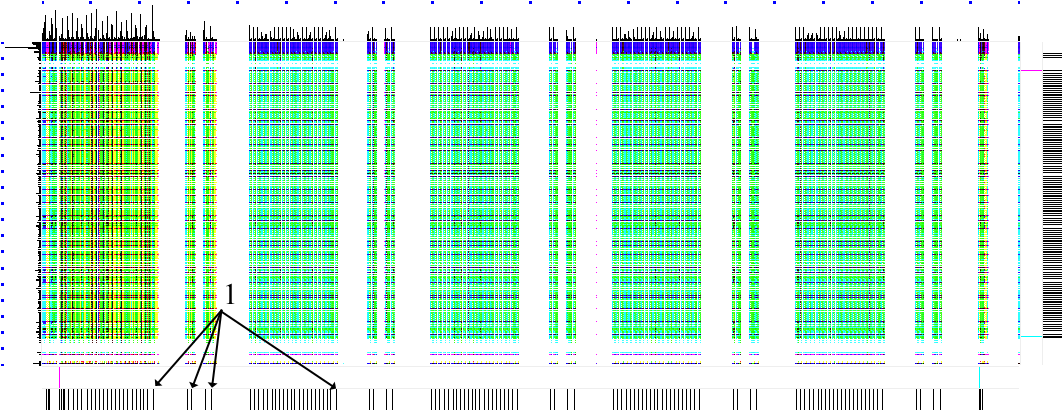
\includegraphics[width=0.7\textwidth]{lviz/wbbench-dp.png}
\end{center}
\caption{Time-ordered VDP comparing IE7 (x-axis) and Chrome (y-axis)
performing the
SunSpider JavaScript benchmark.
}
\label{fig:wbbench-dp}
%\begin{tabular}{ll}
%DP match : & operation\\
%DP color : & cyan $\rightarrow$ file; magenta $\rightarrow$ registry;
%yellow $\rightarrow$ network operation\\
%Bar1 color : & cyan $\rightarrow$ benchmark start time;
%magenta $\rightarrow$ benchmark end time\\
%Bar2 color : & black $\rightarrow$ HTTP GET event
%\end{tabular}
{\it DP match}: operation;
{\it DP color}: cyan $\rightarrow$ file; magenta $\rightarrow$ registry;
yellow $\rightarrow$ network operation;
{\it Bar1 color}: cyan $\rightarrow$ benchmark start time;
magenta $\rightarrow$ benchmark end time;
{\it Bar2 color}: black $\rightarrow$ HTTP GET event.
\end{figure}

We use time-ordered VDP (Figure~\ref{fig:wbbench-dp}) to investigate the
SunSpider JavaScript benchmarks on
two web browsers, Internet Explorer 7 (IE7) and Google Chrome.
The benchmark consists of 26 different tests repeated for 5 times.
Since the browser fetches a web page for each test,
we use the HTTP GET\footnote{
To mark HTTP GET events, we need to turn on network data I/O collection
and use a suitable regular expression as the barcode coloring rule.
The start and end events are marked by matching the two URLs.
}
event (shown in Bar2) to mark the beginning
of each test.
By looking at the time-ordered DP, we know that Chrome is about three
times faster than IE7 in total and also in each test.
From Bar2,
we can also observe that some tests (followed by long white gap,
pointed by marker 1) take much longer time than others.
By clicking on those events, we found out the slow ones to be all string
operation\footnote{
The URLs are \url{/perf/sunspider-0.9/string-base64.html},
\url{/perf/sunspider-0.9/string-tagcloud.html},
and \url{/perf/sunspider-0.9/string-validate-input.html}}
benchmarks.
We conclude that one reason why IE7 is slower than Chrome is due to string operations.

%\input{lviz/ex-iexploit}
%\input{lviz/ex-virus}

\subsection{Conclusion}
\label{sec:lviz-conclusion}

The objective of this work is twofold.
Firstly, we show that visualization can be beneficial for problems
in software understanding and diagnosis. We demonstrate this
for traces with a single program as well as with
several programs and a complete system trace.
Secondly, we show that a DotPlot-based visualization, VDP, is effective
in visualizing a range of problems.
One feature which distinguishes \code{lviz} is that as we work
at the operating system level with system and stack traces,
we do not need source code of the software.
We believe that the range of understanding and diagnosis applications
shows that visualization of operating system traces is an interesting approach.
It also complements other kinds of analysis such
as program analysis and data mining.

Our VDP visualization is only one general purpose visualization.
There are some other problems where dependency visualizations
(Section~\ref{sec:depvis}) or special
variants of VDP would be more appropriate. For example, to understand
resource usage, a special kind of VDP with resources and traces overlaid
with resource lifetimes would give more information than a regular VDP.
We have not taken advantage of source code and this can further enhance
the visualization but it would need monitoring infrastructure which
can correlate execution with the source.
We also remark that although we do not make use of source code, we
see that visualizations using program points can be used to understand
how the code works (at the native code level).

We have developed the VDP tool for Windows because such visualizations
are more beneficial given the closed source nature and system complexity
of Windows.
However, VDP is not reliant on a particular monitoring infrastructure
as the input trace format is very simple.
The same visualization ideas can be applied
to other systems with a rich source of execution traces, e.g. UNIX variants.

